\documentclass{article}
\usepackage{cmap}
\usepackage[T2A]{fontenc}
\usepackage[utf8]{inputenc}
\usepackage[english,russian]{babel}
\usepackage{setspace}
\usepackage{geometry}
\usepackage{graphicx}
\graphicspath{{graphicslab1/}}
\DeclareGraphicsExtensions{.pdf, .png, .jpg, .fig}
\geometry{top=2cm}
\geometry{bottom=2cm}
\geometry{left=2cm} % отступ справа
\geometry{right=2cm} % отступ слева

\begin{document}
	\begin{center}
		\hfill \break
		\begin{center}
			\huge{Санкт-Петербургский политехнический университет\\
				Высшая школа прикладной математики\\
				и вычислительной физики, ФизМех}
		\end{center}
		\hfill \break
		\hfill \break
		\hfill \break
		\hfill \break
		\hfill \break
		\huge{Направление подготовки\\
			«Прикладная математика и информатика»}\\
		\hfill \break
		\hfill \break
		\hfill \break
		\hfill \break
		\hfill \break
		\hfill \break
		\fontsize{14pt}{14pt}\selectfont
		Отчет по лабораторной работе №1\\
		«Решение алгебраических и трансцендентных уравнений»\\
		\hfill \break
		\hfill \break
		\hfill \break
		\hfill \break
		\hfill \break
	\end{center}
	\hfill \break
	\hfill \break
	\fontsize{12pt}{12pt}\selectfont
	\begin{tabular}{cccc}
		\hspace{1cm}Выполнил студент гр. 5030102/00003 & {\hspace{3cm}} & & Петрошенко А.В. \\\\
		\hspace{-3cm}Преподаватель: &{\hspace{1cm}}& & {\hspace{1cm}} Курц В.В. \\\\
	\end{tabular}\\
	\hfill \break
	\hfill \break
	\hfill \break
	\hfill \break
	\hfill \break
	\hfill \break
	\begin{center} Санкт-Петербург\\ 
	2021\\
	\end{center}
	\thispagestyle{empty}
	\newpage
	\begin{center} \textbf{Формулировка задачи и ее формализация}\end{center}
	Существует 2 метода решения алгебраических и трансцендентных уравнений: аналитические методы и численные. К сожалению, класс уравнений, решаемых с помощью аналитических довольно узок. Основные проблемы:\\
	-Алгебраические разрешими только до 4-ой степени.\\
	-Трансцендентные в общем случае неразрешимы.\\
	-Заранее неизвестно, есть ли корни и сколько их.\\
	Решение делится на 2 этапа:\\
	Этап отделения - нахождения отрезков, на которых лежит только 1 корень данной функции.\\
	Этап уточнения - нахождение этого корня с точностью $\epsilon$.\\
	\\
	\underline{Формализация задачи:}\\
	\\
	Пусть есть $f(x): R\rightarrow R$ – алгебраическая или трансцендентная функция одной переменной. Требуется найти такой $x^*: f(x^*) = 0$ с помощью двух численных методов и сравнить их эффективность.\\
	\\
	\underline{Поставленные задачи:}\\
	\\
	1. Найти промежуток переменной \textit{x}, который содержит лишь один корень и удовлетворяет условиям применимости численных методов:\\
	метода половинного деления и модифицированного метода Ньютона\\
	\\
	2. Применить данные численные методы для решения двух уравнений (алгебраического и трансцендентного):
	\begin{center} $x^5 + x^2 - 5 = 0$\\
		$5^x + 3x = 0$\\
	\end{center}
	3. Сравнить полученные нами ответы с ответами, полученными с помощью средств пакета MATLAB.\\
	\\
	4. Построить графики и сравнить эффективность данных численных методов:\\
	График сходимости методов\\
	График зависимости объема вычислений от точности получаемого значения\\
	График, показывающий достигнута ли нужная точность\\
	График зависимости объема вычислений от первого приближения(Модифицированный метод Ньютона)\\
	\newpage
	\begin{center} \textbf{Алгоритмы методов и условия их применимости}\end{center}
	\underline{Метод 1: Метод половинного деления}\\
	\\
	Пусть у нас есть отрезок $[a, b]$, на котором определена и имеет единственный корень $x^*$ функция $f$.\\
	\\
	Условия применимости метода:\\
	1. $f \in C([a, b])$ (функция непрерывна)\\
	2. $f(a)f(b) < 0$\\
	\\
	Алгоритм метода:\\
	while ($|b - a| > 2\epsilon$)\\
	\{\\
	\hspace*{1cm} $c = \frac{a+b}{2}$;\\
	\hspace*{1cm} if($f(a)f(b) < 0$)\\
	\hspace*{2cm} b = c;\\
	\hspace*{1cm} else\\
	\hspace*{2cm} a = c;\\
	\}\\
	$x = \frac{a+b}{2}$;\\
	\\
	\underline{Метод 2: Модифицированный метод Ньютона}\\
	\\
	Пусть у нас есть отрезок $[a, b]$, на котором определена и имеет единственный корень $x^*$ функция $f$, а также начальное приближение $x_0$.\\
	\hfill \break
	Условия применимости метода:\\
	1. $f \in C^2([a, b])$ (функция и ее первые две производные непрерывны)\\
	2. $f(a)f(b) < 0$\\
	3. $f'(x), f''(x)$ знакопостоянны\\
	4. $f(x_0)f''(x_0) > 0$\\
	\textbf{Замечание.} Проблема последнего пункта в том, что $\exists x_0\in [a, b]: f(x_0)f''(x_0) < 0$, поэтому при реализации методов мы отдельно берем промежуток где данное условие выполняется.\\
	\\
	Алгоритм метода:\\
	$x_k = x_0$;\\
	while ($f(x_k + \epsilon)f(x_k - \epsilon) > 0$)\\
	\{\\
	\hspace*{1cm} $x_{k-1}= x_k$;\\
	\hspace*{1cm} $x_k = \frac{f(x_{k-1})}{f'(x_0)}$;\\
	\}\\
	\\
	Отказ от высчитывания производной на каждой итерации позволяет сократить время, но падает скорость сходимости. Для ускорения сходимости значение производной можно пересчитывать после нескольких итераций. Мы будем пересчитывать каждую вторую итерацию.\\
	\newpage
	\begin{center} \textbf{Предварительный анализ задачи}\end{center}
	\underline{Алгебраическая функция:}
	$x^5 + x^2 - 5 = 0$\\
	$\triangleright$ Верхние и нижние границы корней:\\
	Для положительных корней: $x^* \le 1 + \sqrt[m]{\frac{|a'|}{a_0}}$\\
	Верхняя граница:\\
	$x^* \le 1 + \sqrt[5]{\frac{5}{1}} \simeq 2.38$\\ 
	Нижняя граница: (замена $x^* = \frac{1}{y})$\\
	$y \le 1 + \sqrt[2]{\frac{1}{5}} \simeq 1.45$\\
	$x \ge 0.69$\\
	Получаем, что для положительных корней $x^* \in [0.69, 2.38]$\\
	\\
	Для отрицательных корней:\\
	Верхняя граница (замена $x^* = -\frac{1}{y}$):\\
	$y \le 1 + \sqrt[2]{\frac{1}{5}} \simeq 1.45$\\
	$x \le -0.69$\\
	Нижняя граница (замена $x^* = -y$):\\
	$y \le 1 + \sqrt[3]{\frac{1}{1}} = 2$\\
	$x \ge -2$\\
	Получаем, что для отрицательных корней $x^* \in [-2, -0.69]$\\
	\\
	$\triangleright$ Условия применимости методов:\\
	Метод половинного деления:\\
	1. $f(x) \in C([1, 2])$\\
	2. $f(1)f(2) < 0\ (-3 \cdot 31 < 0)$\\
	\\
	Модифицированный метод Ньютона:\\
	1. $f(x) \in C^2([1, 2])$\\
	2. $f(1)f(2) < 0$\\
	3. $f'(x) и f''(x)$ знакопостоянны (обе положительны)\\
	4. Для $x_0$ сужаем промежуток до $[1.5, 2]$, то есть $\forall x_0 \in [1.5, 2]\ f(x_0)f''(x_0) > 0$\\
	\\
	Все условия применимости выполнены, значит, можем применять методы на данном промежутке\\
	\\
	\underline{Трансцендентная фукнция:}
	$5^x + 3x = 0$\\
	$\triangleright$ Промежуток\\
	Воспользуемся графическим методом и возьмем промежуток $[-1, 2]$\\ 
	$\triangleright$ Условия применимости методов:\\
	Метод половинного деления:\\
	1. $f(x) \in C([-1, 1])$\\
	2. $f(-1)f(1) < 0\ (-2.8 \cdot 8 < 0)$\\
	\\
	Модифицированный метод Ньютона:\\
	1. $f(x) \in C^2([-1, 1])$\\
	2. $f(-1)f(1) < 0$\\
	3. $f'(x) и f''(x)$ знакопостоянны (обе положительны)\\
	4. Для $x_0$ сужаем промежуток до $[0, 1]$, то есть $\forall x_0 \in [0, 1]\ f(x_0)f''(x_0) > 0$\\
	\\
	Все условия применимости выполнены, значит, можем применять методы на данном промежутке\\
	\\
	\newpage
	\begin{center} \textbf{Тестовый пример для задачи малой размерности}\end{center}
	\underline{Функция:} $f(x) = x^2 + 3x - 2 = 0$ на $[-1, 1]$, $\epsilon = 0.01$\\
	$\triangleright$ Метод половинного деления:\\
	$f(x) \in C([-1, 1])$\\
	$f(-1)f(1) < 0$\\
	Расчеты:
	\begin{enumerate}
		\item $[-1, 1]:$ $f(a) = -4$, $f(b) = 2$, $f(c) = -2$, $f(a)f(c) > 0$
		\item $[0, 1]:$ $f(a) = -2$, $f(b) = 2$, $f(c) = -0.25$, $f(a)f(c) > 0$
		\item $[0.5, 1]:$ $f(a) = -0.25$, $f(b) = 2$, $f(c) = 0.813$, $f(a)f(c) < 0$
		\item $[0.5, 0.75]:$ $f(a) = -0.25$, $f(b) = 0.813$, $f(c) = 0.266$, $f(a)f(c) < 0$
		\item $[0.5, 0.625]:$ $f(a) = -0.25$, $f(b) = 0.266$, $f(c) = 0.004$, $f(a)f(c) < 0$
		\item $[0.5, 0.5625]:$ $f(a) = -0.25$, $f(b) = 0.004$, $f(c) = -0.124$, $f(a)f(c) > 0$		
		\item $[0.5313, 0.5625]:$ $f(a) = -0.124$, $f(b) = 0.004$, $f(c) = -0.06$, $f(a)f(c) > 0$
	\end{enumerate}
	$|b - a| = 0.5625 - 0.5469 = 0.0156 < 2\epsilon$ $\rightarrow$ $x^* = 0.5547$\\
	Мы получили ответ с точностью $\epsilon = 0.01$ за 7 итераций\\
	$\triangleright$ Модифицированный метод Ньютона:\\
	$f(x) \in C^2([-1, 1])$\\
	$f(-1)f(1) < 0$\\
	$f'(x),f''(x)$ знакопостоянны\\
	Возьмем первое приближение $x_0 = 1$, Тогда $f(x_0)f''(x_0) > 0$\\
	Расчеты:\\
	$f'(x_0) = 5$
	\begin{enumerate}
		\item $x_{k-1} = 1$, $x_k = 1 - \frac{2}{5} = 0.6$, $f(0.61)f(0.59) > 0$
		\item $x_{k-1} = 0.6$, $x_k = 0.6 - \frac{0.16}{5} = 0.568$, $f(0.558)f(0.578) < 0$
	\end{enumerate}
	Таким образом, мы получаем, что $x^* = 0.568$ всего за 2 итерации, что в 3.5 раза быстрее, чем методом половинного деления.
	\begin{center} \textbf{Контрольные тесты}\end{center}
	\begin{enumerate}
		\item $f(x) = x^5 + x^2 - 5, x \in [1, 2]$. Мы будем изменять точность $\epsilon$ с $10^{-1}$ до $10^{-15}$ с шагом в 0.1
		\item $f(x) = 5^x + 3x, x \in [-1, 1]$. Мы будем изменять точность $\epsilon$ с $10^{-1}$ до $10^{-15}$ с шагом в 0.1
		\item $f(x) = x^5 + x^2 - 5$. Поменяем промежуток $[1, 2]$ на $[1.5, 2]$, чтобы выполнялось последнее условие применимости метода Ньютона. Расширим новый промежуток до $[1.5, 60]$ и будем брать первое приближение $x_0$ из данного промежутка с шагом 0.05. Точность оставим равной $\epsilon = 10^{-15}$.
		\item $f(x) = 5^x + 3x$. Поменяем промежуток $[-1, 1]$ на $[0, 1]$, чтобы выполнялось последнее условие применимости метода Ньютона. Расширим новый промежуток до $[0, 50]$ и будем брать первое приближение $x_0$ из данного промежутка с шагом 0.05. Точность оставим равной $\epsilon = 10^{-15}$.
		\item $f(x) = x^5 + x^2 - 5$. Будем изменять промежуток с $[1, 2]$ до $[1, 60]$ с шагом 1. Точность оставим равной $\epsilon = 10^{-15}$.
		\item $f(x) = 5^x + 3x$. Будем изменять промежуток с $[-1, 1]$ до $[-1, 50]$ с шагом 1. Точность оставим равной $\epsilon = 10^{-15}$.
	\end{enumerate}
	\newpage
	\begin{center} \textbf{Модульная структура}\end{center}
	\verb|double Complex_Func(double x)|\\
	\verb|double Polynom(double x)|\\
	Это 2 данные фукнции, трансцендентная и полином, то есть алгебраическая..\\
	\\
	\verb|double first_derivative(double x, double (*Func)(double))| - возвращает значение производной принятой на вход функции в выбранной точке.\\
	\\
	\verb|double first_approximation(double a, double b)| - возвращает псевдо-случайное значение из заданного промежутка\\
	\\
	\verb|vector<double> Fzero_bisection(double a, double b, double epsilon,|\\ \verb|double (*Func)(double))|\\
	\verb|vector<double> Fzero_mod_Newton(double a, double b, double epsilon,|\\ \verb|double (*Func)(double))|\\
	Реализация 2-х данных методов. Принимают на вход промежуток, точность и функцию, корень которой нужно найти. Возвращает массив из значений на каждой итерации.\\
	\\
	\verb|void Influence_of_first_approximation_n(double a, double b, double epsilon,|\\
	\verb|double (*Func)(double), const char* filename)|\\
	\verb|void Influence_of_first_approximation_hd(double a, double b, double epsilon,|\\
	\verb|double (*Func)(double), const char* filename)|\\
	Отдельные функции для записи в файл данных, нужных для анализа зависимости количества итераций от первого приближения.\\
	\\
	\verb|void Output(vector<double> vec, double epsilon, const char* filename)|\\
	Функция для записи в файл данных: точности, количества итераций, конечного ответа и значений на каждой итерации.
	\begin{center} \textbf{Численный анализ}\end{center}
	\textit{Комментарий:} Дальнейший анализ производится при точности $\epsilon = 10^{-15}$\\
	$\triangleright$ Значения корней:\\
	\underline{Алгебраическая функция:}\\
	По методу половинного деления - $x^* = 1.2753$(49 итераций)\\
	По модифицированному метода Ньютона - $x^* = 1.2753$(9 итераций)\\
	\\
	\underline{Трансцендентная функция:}\\
	По методу половинного деления - $x^* = -0.2301$(50 итераций)\\
	По модифицированному метода Ньютона - $x^* = -0.2301$(7 итераций)\\
	\\
	\textbf{Небольшой вывод.} Метод Ньютона, очевидно, сходится на порядок быстрее метода половинного деления, как и ожидалось.\\
	\\
	\newpage
	\hspace*{-0.65 cm} $\triangleright$ Достижение нужной точности:\\
	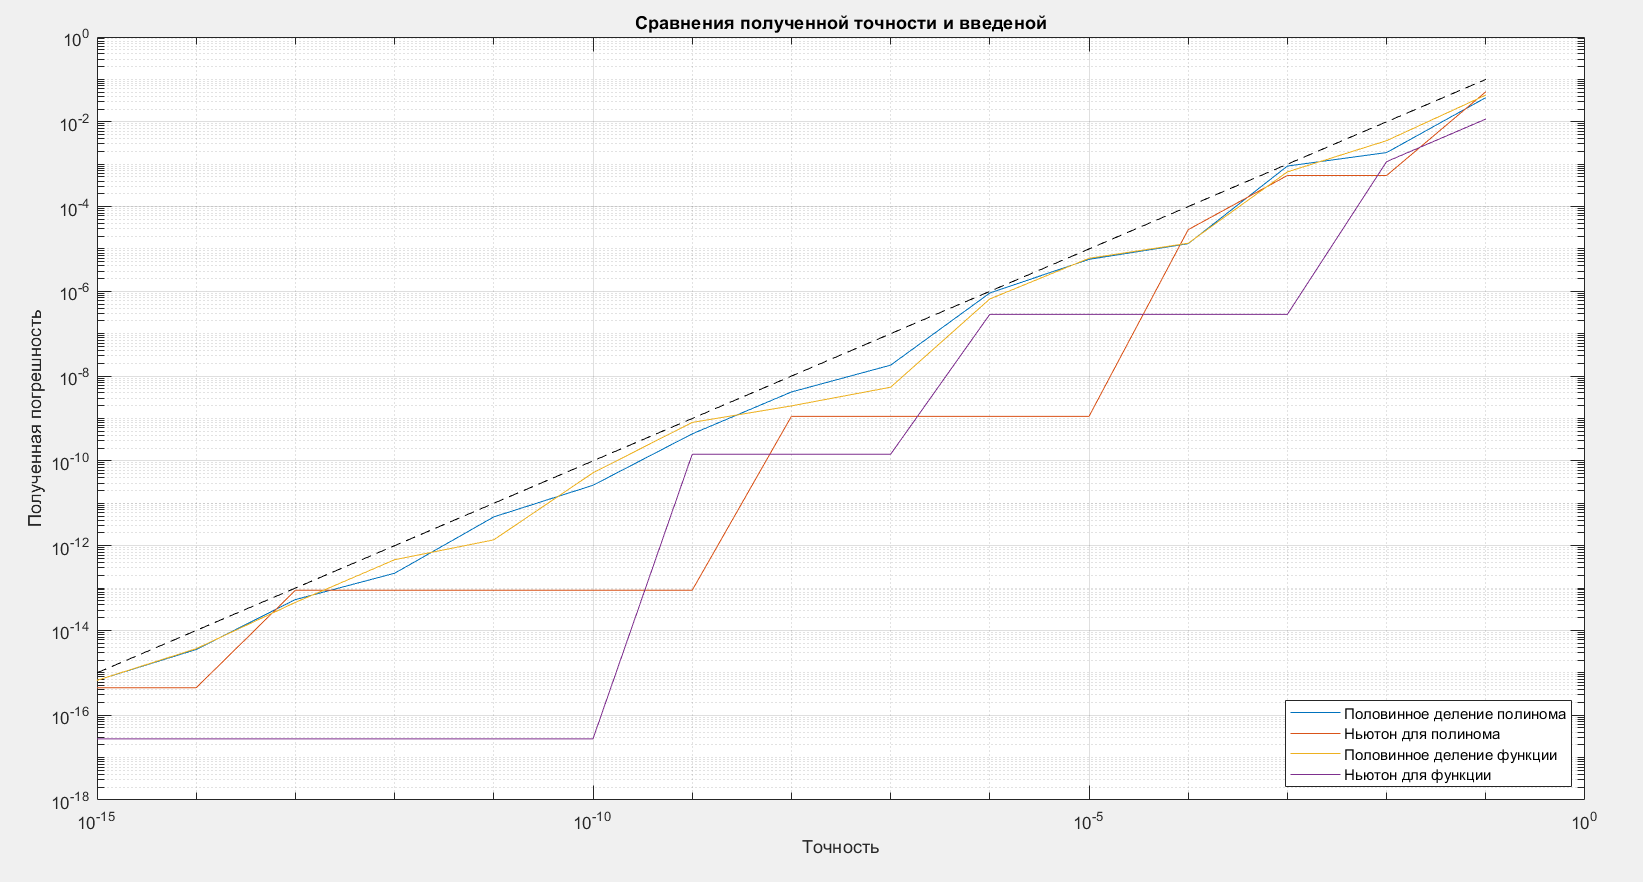
\includegraphics[scale = 0.41]{Сравнение точности}\\
	Сравнив полученные ответы с функцией fzero в MATLAB'е, мы получили погрешность, в среднем, на порядок меньшую заданной точности, значит, все ответы получены верно.\\
	\\
	$\triangleright$ Сходимость:\\
	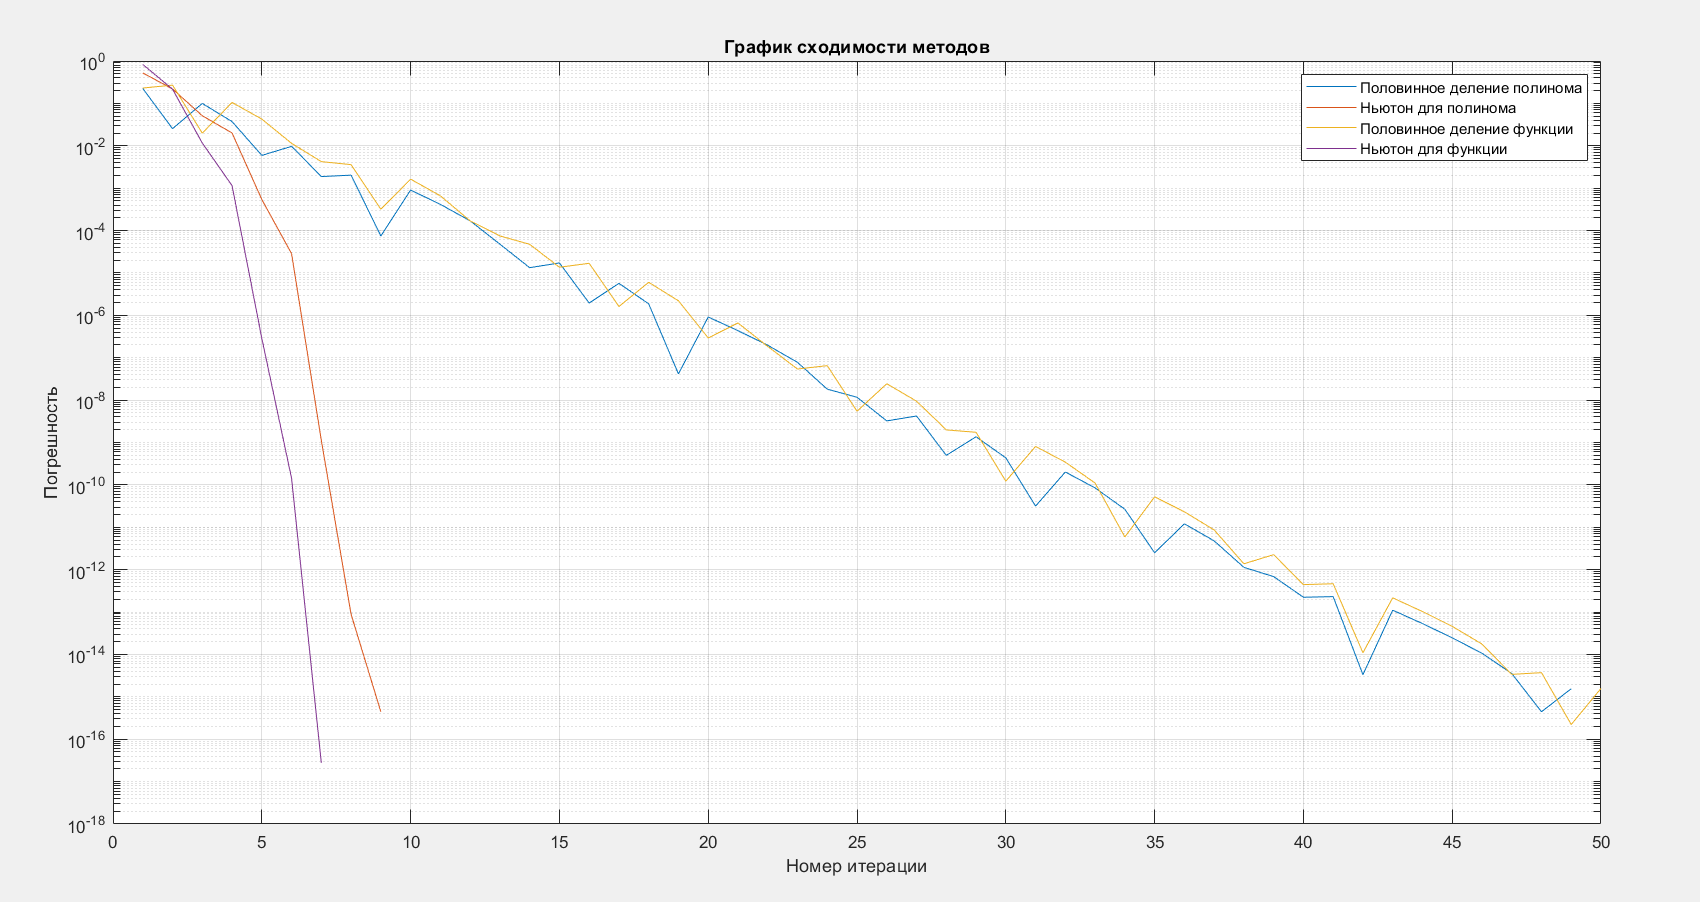
\includegraphics[scale = 0.4]{Сходимость}\\
	Метод половинного деления имеет линейную сходимость. Также отсутствует монотонность, что тоже ожидаемо, т.к. условие выхода из цикла не зависит от того, насколько мы близки к корню\\
	Модифицированный метод Ньютона имеет квадратичную сходимость, при чем сходится монотонно.\\
	\\
	\newpage
	\hspace*{-0.65 cm} $\triangleright$ Объем вычислений:\\
	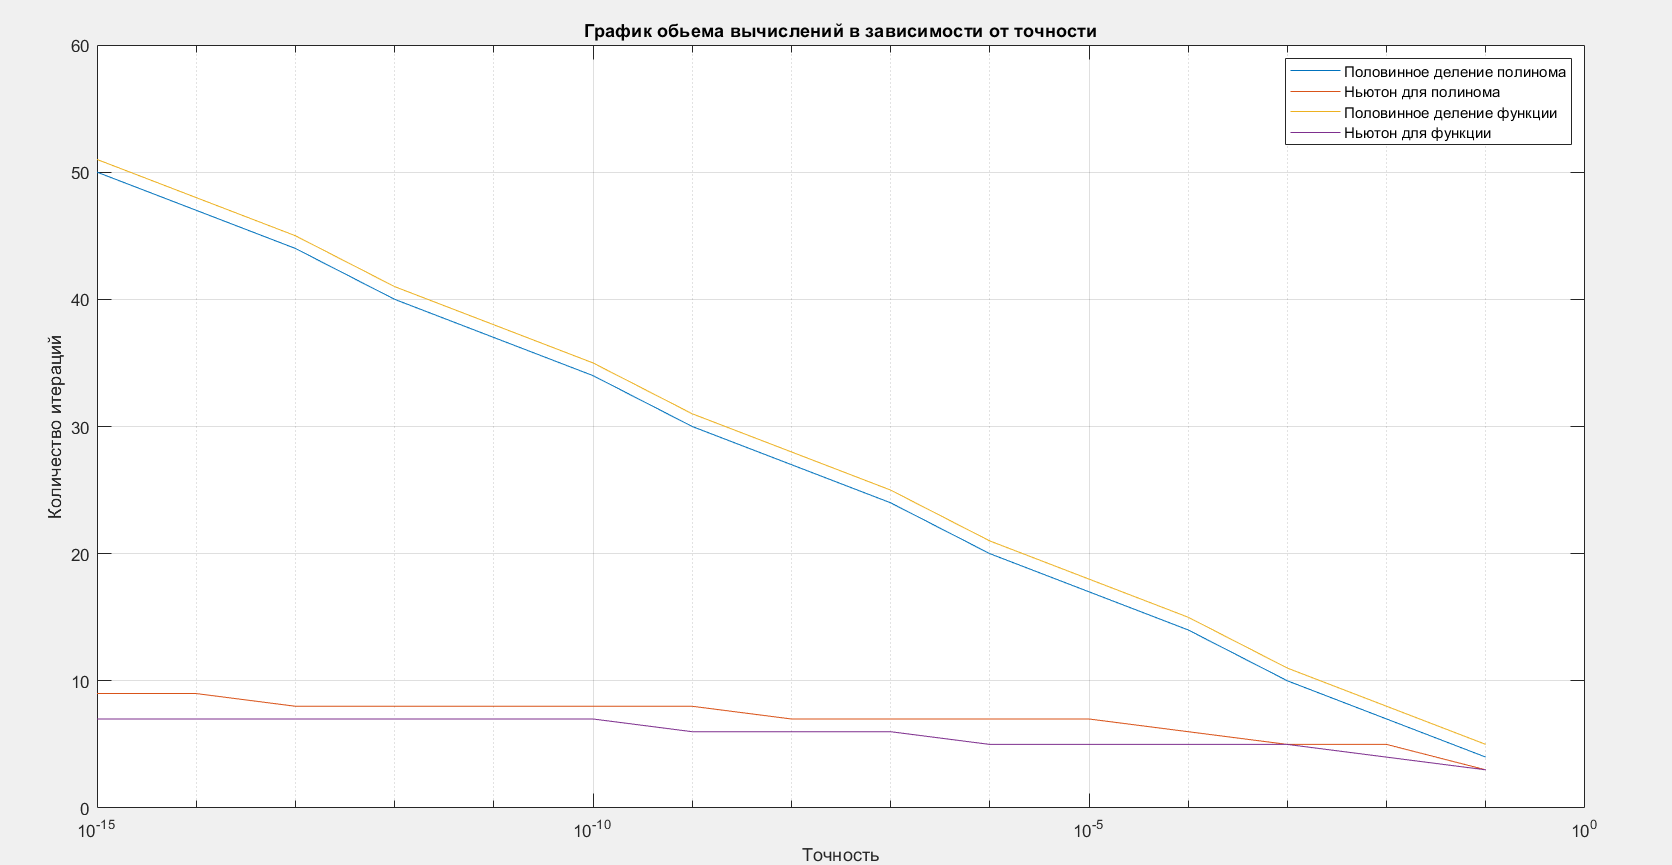
\includegraphics[scale = 0.41]{Объем вычислений}\\
	Аналогично сходимости Метод половинного деления имеет линейную зависимость от точности, а метод Ньютона - квадратичную.\\
	\\
	$\triangleright$ Зависимость количества итераций от первого приближения:\\
	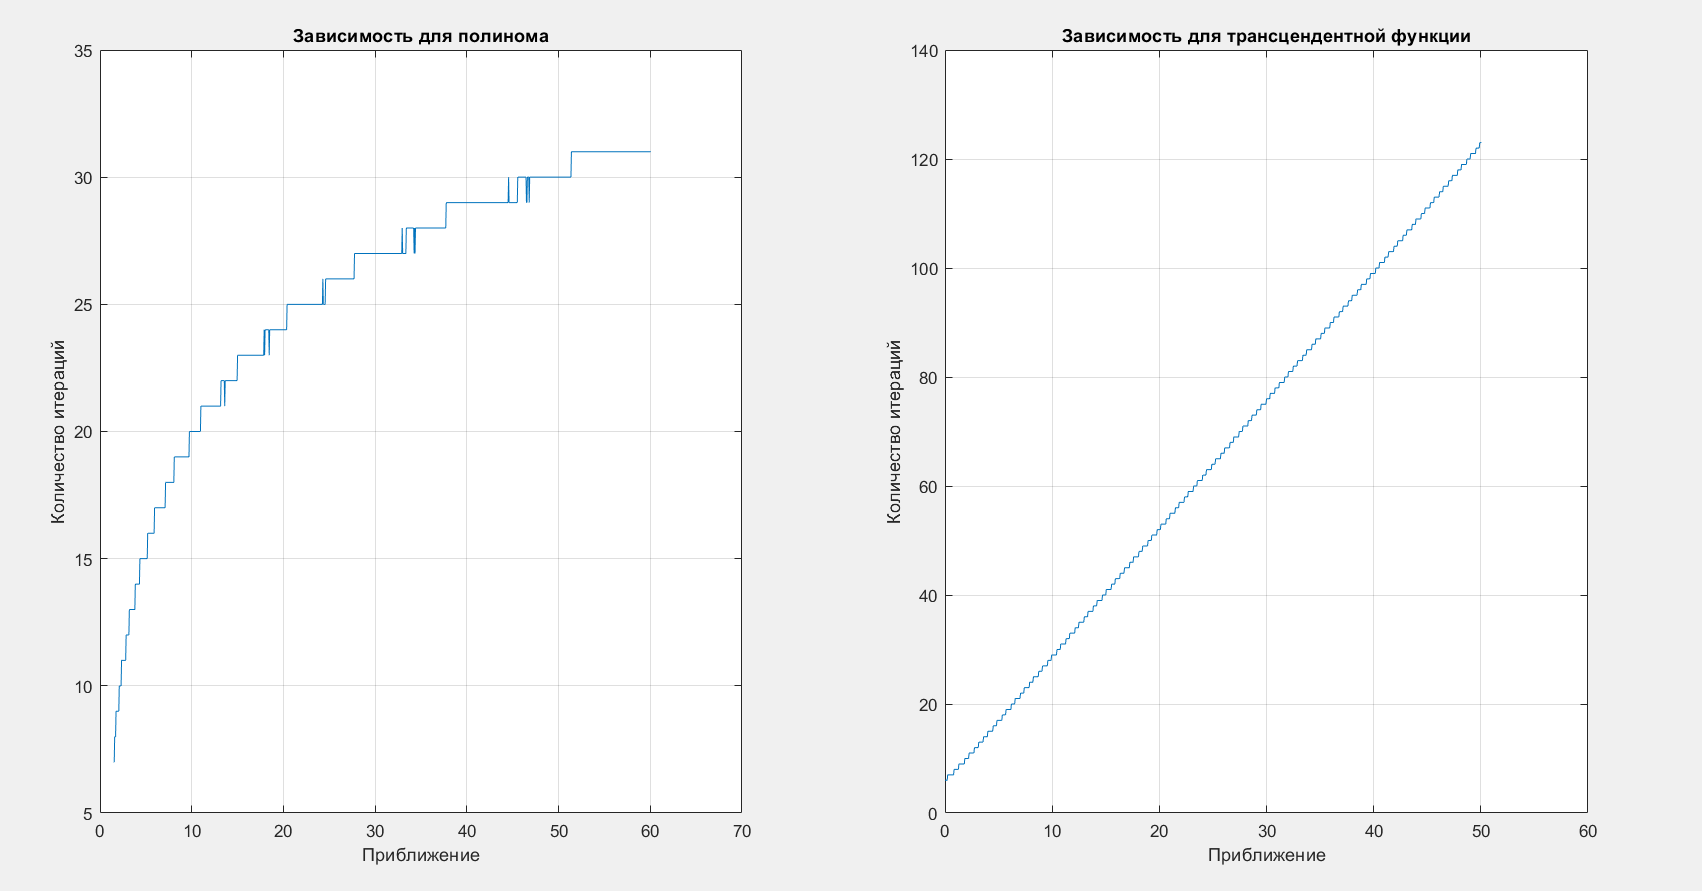
\includegraphics[scale = 0.2]{Приближения Ньютон}
	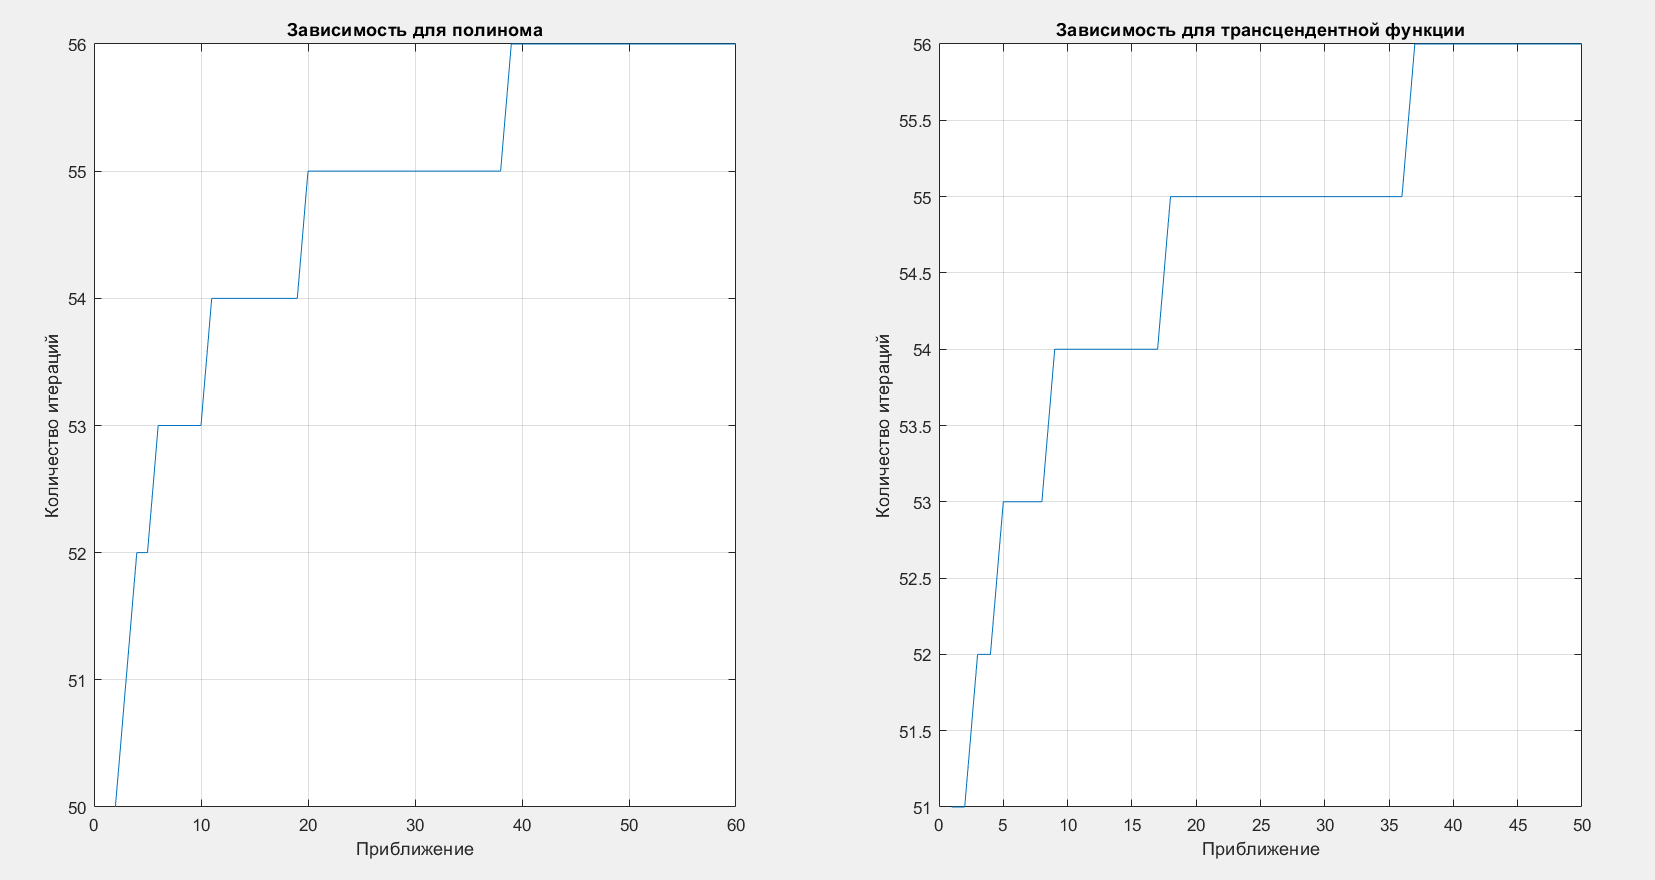
\includegraphics[scale = 0.2]{Приближения МПД}\\
	Для метода половинного деления все стабильно - линейность.
	Для метода Ньютона зависимости для полинома и для трансцендентной функции различны:\\
	Для полинома график повторяет график функции $y = \sqrt{x}$, а для трансцендентной функции зависимость линейная.\\
	\begin{center} \textbf{Общие выводы}\end{center}
	В данной лабораторной работе мы научились находить корни алгебраической и трансцендентной функций 2-мя методами: половинного деления и Ньютона, сравнили их эффективность. Определили, что независимо от вида функции метод половинного деления стабильно сходится к корню, а метод Ньютона сходится гораздно быстрее, но в зависимости от вида функции и первого приближения может иметь не прямо пропорциональный объем вычислений.\\
	Таким образом, чтобы выбрать наиболее хороший метод для нахождения корня функции, нужно ее детально исследовать, а еще лучше использовать комбинированные методы. 
\end{document}